\documentclass[12pt,a4paper]{article}

% ─── Encoding & Language ───────────────────────────────────────────────────────
\usepackage[utf8]{inputenc}
\usepackage[T1]{fontenc}
\usepackage[italian]{babel}

% ─── Fonts ─────────────────────────────────────────────────────────────────────
\usepackage{lmodern}
\usepackage{microtype}

% ─── Mathematics ───────────────────────────────────────────────────────────────
\usepackage{amsmath}
\usepackage{amssymb}

% ─── Graphics & Colors ─────────────────────────────────────────────────────────
\usepackage{graphicx}
\usepackage[table]{xcolor}
\usepackage{tikz}
\usetikzlibrary{shapes.geometric, arrows.meta, positioning, calc}

% ─── Layout ────────────────────────────────────────────────────────────────────
\usepackage[
  a4paper,
  left=30mm, right=30mm,
  top=30mm, bottom=20mm,
  headheight=25pt,
  footskip=10mm
]{geometry}
\usepackage{float}
\usepackage{parskip}
\usepackage{setspace}
\setstretch{1.18}

% Palette: tutto in scala di grigi/antracite — niente colori accesi
\definecolor{titlecolor}{RGB}{30, 30, 30}      % quasi nero per i titoli
\definecolor{rulecolor}{RGB}{100, 100, 100}    % grigio medio per le righe
\definecolor{muted}{RGB}{130, 130, 135}        % grigio per elementi secondari
\definecolor{codebg}{RGB}{248, 248, 246}       % sfondo code molto leggero
\definecolor{codeframe}{RGB}{180, 180, 175}    % bordo code grigio tenue
\definecolor{codegreen}{RGB}{50, 120, 60}
\definecolor{codepurple}{RGB}{100, 30, 130}
\definecolor{codeblue}{RGB}{30, 60, 140}
\definecolor{codegray}{RGB}{120, 120, 120}
\definecolor{boxbg}{RGB}{240, 240, 240}        % sfondo box leggermente più scuro
\definecolor{boxframe}{RGB}{80, 80, 80}        % bordo box scuro per contrasto

% ─── Headers & Footers ─────────────────────────────────────────────────────────
\usepackage{fancyhdr}
\pagestyle{fancy}
\fancyhf{}
\fancyhead[R]{\small\textcolor{muted}{Simulatore C3 Queueing System}}
\fancyfoot[C]{\small\textcolor{muted}{\thepage}}
\renewcommand{\headrulewidth}{0.4pt}
\renewcommand{\headrule}{%
  \hbox to\headwidth{\color{rulecolor}\leaders\hrule height \headrulewidth\hfill}}

% ─── Section Styling ───────────────────────────────────────────────────────────
\usepackage{titlesec}

\titleformat{\section}
  {\large\bfseries\color{titlecolor}}
  {\thesection.}{0.6em}{}
  [\vspace{-0.25em}\textcolor{rulecolor}{\rule{\linewidth}{0.5pt}}]

\titleformat{\subsection}
  {\normalsize\bfseries\color{titlecolor}}
  {\thesubsection.}{0.5em}{}

\titleformat{\subsubsection}
  {\normalsize\itshape\color{muted}}
  {\thesubsubsection.}{0.5em}{}

\titlespacing*{\section}{0pt}{2em}{0.7em}
\titlespacing*{\subsection}{0pt}{1.3em}{0.35em}
\titlespacing*{\subsubsection}{0pt}{0.9em}{0.2em}

% ─── Table of Contents ─────────────────────────────────────────────────────────
\usepackage{tocloft}
\renewcommand{\cftsecfont}{\bfseries}
\renewcommand{\cftsecpagefont}{\bfseries}
\renewcommand{\cfttoctitlefont}{\large\bfseries\color{titlecolor}}
\setlength{\cftbeforesecskip}{4pt}

% ─── Code Listings ─────────────────────────────────────────────────────────────
\usepackage{listings}
\lstdefinestyle{cppstyle}{
  backgroundcolor=\color{codebg},
  commentstyle=\itshape\color{codegreen},
  keywordstyle=\bfseries\color{codeblue},
  numberstyle=\tiny\color{codegray},
  stringstyle=\color{codepurple},
  basicstyle=\ttfamily\small,
  breakatwhitespace=false,
  breaklines=true,
  captionpos=b,
  keepspaces=true,
  numbers=left,
  numbersep=10pt,
  showspaces=false,
  showstringspaces=false,
  showtabs=false,
  tabsize=2,
  frame=single,
  framesep=6pt,
  xleftmargin=16pt,
  xrightmargin=4pt,
  rulecolor=\color{codeframe},
  framerule=0.5pt,
  aboveskip=1em,
  belowskip=1em
}
\lstset{style=cppstyle}

% ─── Hyperlinks ────────────────────────────────────────────────────────────────
\usepackage{hyperref}
\hypersetup{
  colorlinks=true,
  linkcolor=titlecolor,
  urlcolor=muted,
  citecolor=muted,
  pdfauthor={Studente},
  pdftitle={Relazione Finale -- Simulatore C3 Queueing System}
}

% ─── Boxes ─────────────────────────────────────────────────────────────────────
\usepackage{tcolorbox}
\tcbuselibrary{skins, breakable}
\newtcolorbox{infobox}[1][]{
  enhanced,
  colback=boxbg,
  colframe=boxframe,
  fonttitle=\bfseries\small,
  coltitle=white,
  left=8pt, right=8pt, top=5pt, bottom=5pt,
  arc=3pt,
  boxrule=1.2pt,
  title={#1}
}

% ─── Captions ──────────────────────────────────────────────────────────────────
\usepackage[
  font={small,it},
  labelfont={bf},
  labelsep=period
]{caption}

% ─── Enumitem ──────────────────────────────────────────────────────────────────
\usepackage{enumitem}
\setlist[itemize]{
  leftmargin=1.5em,
  itemsep=0.25em,
  label={\textcolor{rulecolor}{\textbullet}}
}
\setlist[enumerate]{
  leftmargin=1.5em,
  itemsep=0.25em,
  label={\textcolor{rulecolor}{\arabic*.}}
}


% ─── Title page ────────────────────────────────────────────────────────────────
\begin{document}

\begin{titlepage}
  \thispagestyle{empty}
  \begin{center}
    \vspace*{4cm}

    {\color{rulecolor}\rule{\linewidth}{0.6pt}}
    \vspace{1.2em}

    {\LARGE\bfseries\color{titlecolor}
      Simulatore Sistema a Code C3}

    \vspace{1.2em}
    {\color{rulecolor}\rule{\linewidth}{0.6pt}}

    \vspace{2.5cm}

    {\normalsize\scshape\color{titlecolor} Progetto Reti e Telecomunicazioni}

    \vspace{0.5cm}
    {\small\color{muted} \today}

    \vfill

    \begin{tcolorbox}[
        enhanced,
        colback=boxbg,
        colframe=boxframe,
        arc=2pt,
        boxrule=0.5pt,
        left=14pt, right=14pt, top=9pt, bottom=9pt,
        width=0.70\textwidth
      ]
      \centering\small\color{muted}
      Davide Bonsembiante - mat. 1086863 \\
      Alessandro Biscaro - mat. 1087892 \\
      Alessandro Rocco - mat. 1081179
    \end{tcolorbox}

    \vspace{2cm}
  \end{center}
\end{titlepage}

% ─── Table of Contents ─────────────────────────────────────────────────────────
\newpage
\tableofcontents
\newpage


\section{Introduzione}


Il progetto \textbf{C3 Queueing System Simulator} è un'applicazione orientata allo studio prestazionale di un modello teorico di code parallele. Il sistema è costituito da $N$ serventi indipendenti, ciascuno dotato di una propria coda \textsc{FIFO} (\textit{First-In-First-Out}) di capacità teoricamente infinita.

\noindent
\textbf{Assunzioni del Modello}

Il modello stocastico adottato soddisfa le seguenti ipotesi:
\begin{itemize}
  \item Gli arrivi al sistema sono regolati da un processo di Poisson con tasso globale $\lambda$.
  \item Ogni pacchetto, appena giunto nel sistema, viene instradato verso una delle $N$ code senza possibilità di preemption né di cambio coda successivo (\textit{no jockeying}).
  \item Il tempo di servizio per il servente $i$-esimo segue una distribuzione esponenziale negativa di media $1/\mu_i$.
\end{itemize}

\noindent
L'obiettivo è valutare e confrontare tre distinte politiche di instradamento in termini di tempo medio di permanenza e indice di bilanciamento del carico, con un'implementazione robusta e ben documentata.

\begin{figure}[H]
  \centering
  \begin{tikzpicture}[
    node distance=1.5cm and 2cm,
    server/.style={circle, draw=boxframe, fill=boxbg, thick, minimum size=1.2cm},
    queue/.style={draw=boxframe, thick, inner sep=0pt, minimum width=2cm, minimum height=0.6cm},
    router/.style={diamond, draw=titlecolor, fill=codebg, thick, aspect=1.5, text centered},
    arrow/.style={-{Stealth[scale=1.2]}, thick, rulecolor}
    ]
    % Router
    \node[router] (dispatch) {Dispatcher};
    \node[left=1.5cm of dispatch] (in) {Arrivi $\lambda$};

    % Servers and Queues
    \node[queue, right=2.5cm of dispatch, yshift=2cm] (q1) {};
    \node[server, right=0cm of q1] (s1) {$\mu_1$};

    \node[queue, right=2.5cm of dispatch] (q2) {};
    \node[server, right=0cm of q2] (s2) {$\mu_2$};

    \node[right=2.5cm of dispatch, yshift=-1cm] (dots) {$\vdots$};

    \node[queue, right=2.5cm of dispatch, yshift=-2cm] (qn) {};
    \node[server, right=0cm of qn] (sn) {$\mu_N$};

    % Queue lines
    \foreach \q in {q1, q2, qn} {
        \draw[thick, boxframe] (\q.south west) -- (\q.south east);
        \draw[thick, boxframe] (\q.north west) -- (\q.north east);
        \draw[thick, boxframe] (\q.north west) -- (\q.south west);
        \draw[thick, boxframe] ($(\q.north west)!0.33!( \q.north east)$) -- ($(\q.south west)!0.33!( \q.south east)$);
        \draw[thick, boxframe] ($(\q.north west)!0.66!( \q.north east)$) -- ($(\q.south west)!0.66!( \q.south east)$);
      }

    % Arrows
    \draw[arrow] (in) -- (dispatch);
    \draw[arrow] (dispatch) -- (q1.west) node[midway, above, sloped, font=\small] {Policy};
    \draw[arrow] (dispatch) -- (q2.west);
    \draw[arrow] (dispatch) -- (qn.west);

    \draw[arrow] (s1.east) -- ++(1,0);
    \draw[arrow] (s2.east) -- ++(1,0);
    \draw[arrow] (sn.east) -- ++(1,0) node[midway, above=0.5cm] {Partenze};
  \end{tikzpicture}
  \caption{Modello architetturale del sistema a code parallele $M/M/N$ implementato.}
  \label{fig:arch_model}
\end{figure}

\newpage
\section{Architettura e Scelte Implementative}

L'applicazione è stata sviluppata interamente in \textbf{C++} con paradigma Object-Oriented (OOP) ed è contenuta nella cartella sorgente \texttt{code/}. È stato adottato un approccio noto come \textit{Discrete Event Simulation} (DES), in cui lo stato del sistema evolve unicamente in corrispondenza di eventi discreti schedulati.

\subsection{Evoluzione rispetto al Modello Base \texorpdfstring{$M/M/1$}{M/M/1}}

Rispetto al codice procedurale di esempio per una singola coda $M/M/1$ analizzato a lezione, questa architettura introduce diverse estensioni fondamentali:
\begin{itemize}
  \item \textbf{Generalizzazione Strutturale:} Il sistema non modella più un singolo servente, ma ospita un vettore dinamico di $N$ oggetti \texttt{Server}, ciascuno dotato del proprio generatore di tempi di servizio esponenziali per la stima indipendente delle partenze.
  \item \textbf{Componente di Routing (Dispatcher):} L'evento \texttt{ARRIVAL} non viene più semplicemente accodato allo stesso nodo. Prima deve attraversare una logica di decisione (\texttt{policy}) che interroga lo stato locale (Round-Robin) o globale (Shortest Queue) del sistema per operare lo smistamento ottimale a runtime.
  \item \textbf{Metriche Distribuite:} L'integrazione a scala temporale (\textit{step-function}) per la lunghezza media della coda, che prima avveniva per un'unica entità, ora viene calcolata perentoriamente in via indipendente su ogni singola istanza \texttt{Server}. Ciò ha reso possibile l'estrazione di indici relazionali (es. sbilanciamento $U$) al termine della simulazione.
\end{itemize}

\subsection{Gestione degli Eventi — \texttt{Event.hpp}}

Ogni cambiamento di stato è modellato come un evento, incapsulato nella \texttt{struct Event}. Esistono due tipi di eventi, denotati dall'\texttt{enum EventType}:

\begin{itemize}
  \item \texttt{ARRIVAL} — arrivo di un nuovo pacchetto dall'esterno.
  \item \texttt{DEPARTURE} — terminazione del servizio da parte di un dato servente.
\end{itemize}

Affinché gli eventi siano estratti in rigoroso ordine cronologico, \texttt{Event} espone l'overload dell'operatore '\texttt{<}' invertito. Inserendo gli eventi in una \texttt{std::priority\_queue}, si ottiene un \textit{min-heap} basato sul timestamp.

\subsection{Modello del Servente — \texttt{Server.hpp}}

La struttura \texttt{Server} memorizza lo stato del singolo nodo, la sua coda specifica (una \texttt{std::queue<double>} contenente i tempi di arrivo dei pacchetti in attesa) e le seguenti metriche di accumulazione:

\begin{itemize}
  \item \texttt{total\_packets\_served} — contatore cumulativo dei pacchetti completati.
  \item \texttt{total\_response\_time} — somma dei tempi di permanenza su quel nodo.
  \item \texttt{area\_queue\_length} — integrale temporale della dimensione della coda, utilizzato per derivare la lunghezza media tramite il Teorema del Valore Medio.
\end{itemize}

\begin{lstlisting}[language=C++, caption={Metodo di calcolo dell'integrale della coda nel tempo (\texttt{Server.hpp}).}, label=lst:server_area]
// Aggiorna l'integrale della coda calcolando l'area del gradino
void update_area(double current_time) {
    area_queue_length += queue.size() * (current_time - last_update_time);
    last_update_time = current_time;
}
\end{lstlisting}

\subsection{Motore di Simulazione — \texttt{Simulator.hpp / .cpp}}

La classe \texttt{Simulator} è il nucleo operativo del progetto e gestisce tre responsabilità principali:

\begin{enumerate}
  \item \textbf{Generazione di Variabili Casuali:}
        Sfrutta l'header \texttt{<random>} del C++. Un generatore Mersenne Twister (\texttt{std::mt19937}) alimenta distribuzioni esponenziali distinte: una per gli arrivi (tasso $\lambda$) e $N$ per i servizi (ciascuna con il proprio $\mu_i$).

  \item \textbf{Ciclo Principale (\texttt{run()}):}
        Schedula il primo arrivo, quindi entra in un ciclo che termina al superamento del parametro \texttt{max\_time}. A ogni iterazione, estrae l'evento imminente e invoca \texttt{handle\_arrival} o \texttt{handle\_departure}, avanzando il \textit{clock} della simulazione e aggiornando le code.

  \item \textbf{Robustezza sull'Input:}
        Se vengono forniti meno valori di $\mu_i$ rispetto a $N$, le entry mancanti vengono inizializzate automaticamente al valore di \textit{fall-back} $\mu_i = 1.0$ (come documentato nei commenti del sorgente).
\end{enumerate}

\subsection{Calcolo delle Metriche}

I KPI richiesti sono derivati rigorosamente durante il ciclo di simulazione:

\begin{itemize}
  \item \textbf{Tempo di permanenza ($W$):}
        All'atto di una partenza, si recupera l'istante di arrivo del pacchetto al nodo. La differenza rispetto al clock corrente costituisce la latenza effettiva; la media si calcola dividendo la somma cumulata per il numero totale di partenze.

  \item \textbf{Lunghezza media della coda:}
        A ogni modifica dello stato di un \texttt{Server}, l'intervallo trascorso $\Delta t$ viene moltiplicato per la dimensione istantanea precedente della coda e sommato all'integrale. Dividendo infine l'area globale per il tempo di simulazione si ottiene la lunghezza media esatta tramite il metodo \textit{step-function}.

  \item \textbf{Indice di sbilanciamento:}
        Differenza formale tra la lunghezza media massima e minima tra gli $N$ serventi al termine della run:
        \[
          U \;=\; \max_{i}\,\bar{L}_i \;-\; \min_{i}\,\bar{L}_i
        \]
\end{itemize}

\section{Logiche di Instradamento}

Il metodo \texttt{Simulator::route\_packet()} implementa le tre policy selezionabili da linea di comando:

\begin{itemize}
  \item \textbf{Random:}
        Estrae un intero da una \texttt{std::uniform\_int\_distribution<int>(0, N-1)}.
        Costo algoritmico: $O(1)$.

  \item \textbf{Round-Robin:}
        Mantiene un indice ciclico persistente nella classe, incrementato tramite aritmetica modulare \texttt{(round\_robin\_index + 1) \% N}.
        Costo algoritmico: $O(1)$.

  \item \textbf{Shortest Queue (JSQ):}
        Applica una scansione \textit{greedy} lineare tra i serventi a ogni arrivo, restituendo l'indice del server con il minor numero di richieste accodate, tenendo conto anche del pacchetto attualmente in elaborazione.
        Costo algoritmico per pacchetto: $O(N)$.
\end{itemize}

Al fine di garantire trasparenza implementativa, di seguito è riportato il codice C++ del metodo \texttt{route\_packet()} che illustra l'instradamento vero e proprio e la risoluzione degli stati di occupazione per il JSQ:

\begin{lstlisting}[language=C++, caption={Logica di selezione del servente per un nuovo arrivo (\texttt{Simulator.cpp}).}, label=lst:routing]
int Simulator::route_packet() {
    switch (policy) {
        case RoutingPolicy::RANDOM:
            return random_server_dist(rng);
            
        case RoutingPolicy::ROUND_ROBIN: {
            int selected = round_robin_index;
            round_robin_index = (round_robin_index + 1) % N;
            return selected;
        }
            
        case RoutingPolicy::SHORTEST_QUEUE: {
            int shortest = 0;
            // Valuta sia la coda che l'eventuale pacchetto in servizio
            size_t min_len = servers[0].queue.size() + (servers[0].is_busy ? 1 : 0);
            for (int i = 1; i < N; ++i) {
                size_t current_len = servers[i].queue.size() + (servers[i].is_busy ? 1 : 0);
                if (current_len < min_len) {
                    min_len = current_len;
                    shortest = i;
                }
            }
            return shortest;
        }
    }
    return 0;
}
\end{lstlisting}


\section{Testing e Campagna Sperimentale}

Per valutare e confrontare le prestazioni delle tre politiche di instradamento al variare del carico, è stata condotta una campagna di test sistematica ed estesa basata sull'esecuzione del simulatore C++. La procedura di raccolta e analisi dei dati segue questi passi:

\begin{enumerate}
  \item \textbf{Compilazione dell'eseguibile:}
        Viene compilato l'eseguibile \texttt{simulator} ottimizzato mediante il comando \texttt{make}.

  \item \textbf{Esecuzione parametrica con Intervalli di Confidenza:}
        Si modula il tasso di arrivo $\lambda \in [5, 14]$ su un sistema base simmetrico composto da $N = 3$ serventi aventi ciascuno $\mu_i = 5$, testando ciascuna delle tre politiche. Al fine di mitigare la varianza stocastica insita nei processi markoviani e garantire validità statistica, vengono eseguite $K = 15$ simulazioni indipendenti per ogni singola configurazione. Da ciascun gruppo di run viene stimata la media campionaria e calcolato l'\textbf{Intervallo di Confidenza al 95\%} sfruttando l'errore standard.

        \newpage
  \item \textbf{Elaborazione dei Risultati e Grafici:}
        I valori medi di tempo di permanenza ($W$) e di sbilanciamento ($U$), corredati dai rispettivi intervalli di confidenza (rappresentati graficamente tramite barre d'errore), sono stati organizzati e tracciati per un'analisi comparativa immediata.
\end{enumerate}

\section{Analisi dei Risultati}

Le figure seguenti illustrano i dati rilevati dalla campagna sperimentale per $\lambda \in [5, 14]$, con capacità totale del sistema $\sum_i \mu_i = 15$.

\subsection{Tempo Medio di Permanenza \texorpdfstring{($W$)}{(W)}}

\begin{figure}[H]
  \centering
  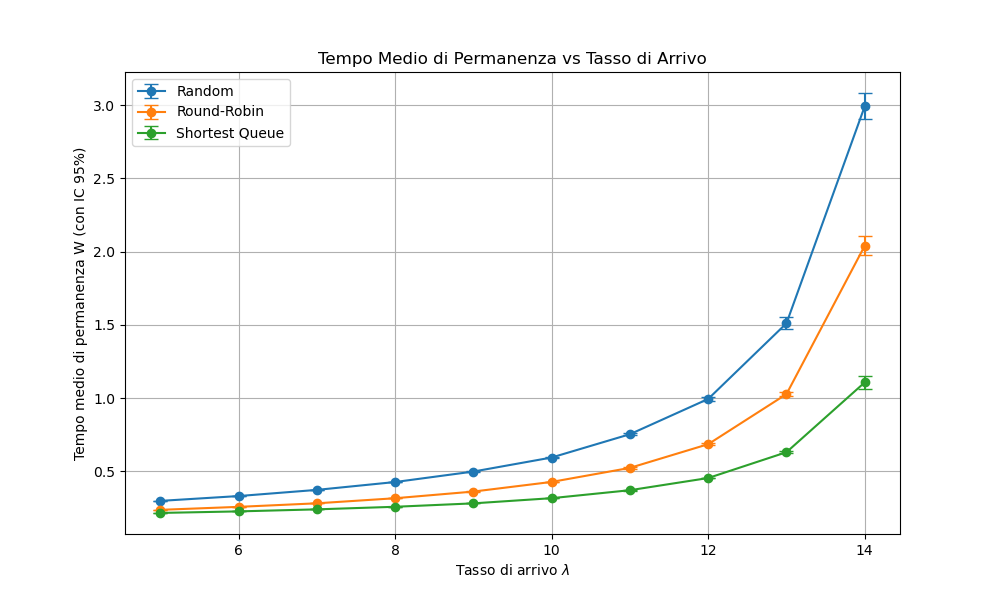
\includegraphics[width=0.78\textwidth]{W_vs_lambda.png}
  \caption{Tempo medio di permanenza nel sistema in funzione del tasso di arrivo $\lambda$.}
  \label{fig:w_vs_lambda}
\end{figure}

Il grafico in Figura~\ref{fig:w_vs_lambda} rivela l'impatto critico dell'algoritmo di assegnazione al saturarsi del sistema ($\sum \mu_i = 15$). In regimi a traffico basso o moderato, \textit{Round-Robin} si avvicina sensibilmente alle prestazioni di JSQ. Tuttavia, ad elevati carichi ($\lambda > 10$), la politica \textit{Random} diviene impraticabile. La \textbf{Shortest Queue} mantiene stabilmente i tempi di permanenza più contenuti: adeguandosi continuamente ai micro-sbilanciamenti in tempo reale, garantisce un utilizzo parallelo ottimale delle risorse.

\subsection{Indice di Sbilanciamento \texorpdfstring{($U$)}{(U)}}

\begin{figure}[H]
  \centering
  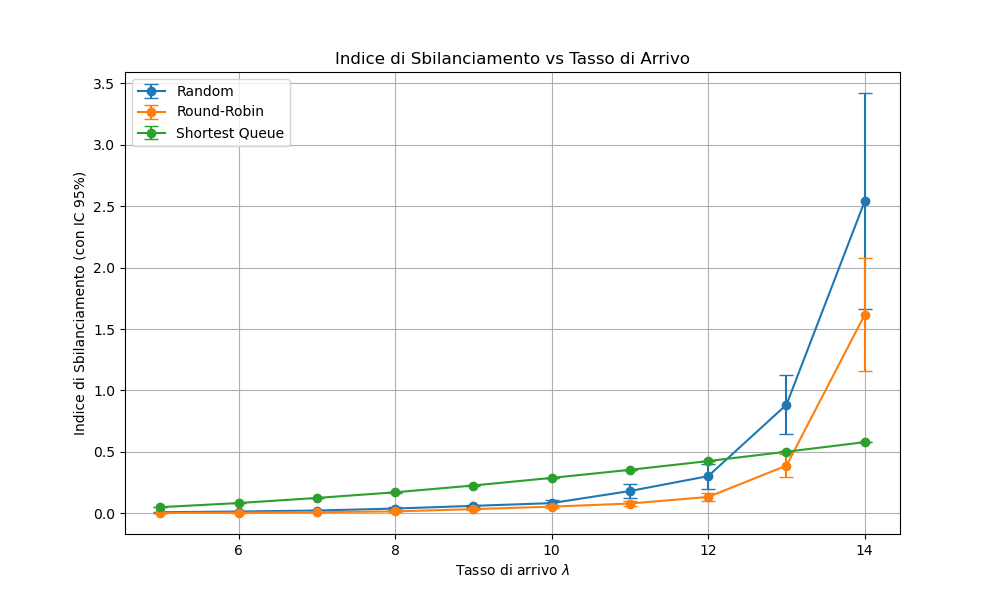
\includegraphics[width=0.78\textwidth]{U_vs_lambda.png}
  \caption{Indice di sbilanciamento $U$ in funzione di $\lambda$.}
  \label{fig:u_vs_lambda}
\end{figure}

La Figura~\ref{fig:u_vs_lambda} mostra una metrica di notevole interesse: per tassi bassi, \textit{Round-Robin} e \textit{Random} producono lunghezze medie statisticamente uniformi, collocandosi vicino a $U \approx 0$. In questo regime JSQ presenta uno sbilanciamento leggermente superiore, intervenendo attivamente a compensare la varianza stocastica degli arrivi.

Al contrario, avvicinandosi alla congestione ($\lambda \approx 14$), le politiche cieche collassano progressivamente. In tale regime, \textbf{JSQ} eccelle anche nello sbilanciamento, mantenendo tutte le code equamente cariche al di sotto di una soglia limitata.

\subsection{Parametrizzazione della Simulazione: Ambienti Eterogenei}

Per studiare il comportamento adattivo e generalizzare i concetti, è possibile alterare la simulazione parametrizzando capacità asimmetriche (eterogenee) tra i serventi, testando così configurazioni non banali.

Ad esempio, modificando i tassi di servizio a linea di comando da una configurazione omogenea $\mu = [5, 5, 5]$ a una sbilanciata \textbf{$\mu = [7, 5, 3]$} (mantenendo identica la capacità di processamento globale $\sum \mu_i = 15$), i risultati si polarizzano.
In tale scenario, policy cieche come \textit{Round-Robin} o \textit{Random} falliscono molto prima, poiché smistano un terzo del traffico incondizionatamente alla velocità del nodo. Il server "lento" ($\mu_3=3$) entra rapidamente in overflow e diventa un insormontabile collo di bottiglia.

Viceversa, la \textbf{Shortest Queue} rivela in questa configurazione il suo reale vantaggio: il server rapido ($\mu_1=7$) smaltisce pacchetti velocemente, rimanendo con la coda frequentemente vuota. Il \textit{Dispatcher JSQ}, osservando l'assenza di congestione, indirizzerà in automatico e naturalmente un volume maggiore di traffico verso questo nodo di fascia alta. Il sistema implementa così una vera e propria forma di \textit{Load-Balancing Dinamico}, autoadattandosi alla potenza di calcolo disomogenea e garantendo stabilità QoS per l'intera sovrastruttura.

\section{Conclusioni}

L'implementazione in C++ si è dimostrata accurata sotto il profilo stocastico e computazionalmente efficiente: le simulazioni ad alta densità di eventi vengono completate in decimi di secondo. Le assunzioni teoriche sui modelli $M/M/1$ accoppiati risultano pienamente supportate:

\begin{itemize}
  \item La politica \textbf{Shortest Queue (JSQ)}, reattiva e deterministica, migliora radicalmente i tempi di risposta (QoS) e ritarda la saturazione in condizioni di traffico elevato.
  \item La politica \textbf{Round-Robin} rappresenta l'alternativa \textit{lightweight} preferibile quando le risorse algoritmiche o la latenza di ispezione risultino vincolate.
\end{itemize}
\end{document}